\documentclass{report}
\usepackage[utf8]{inputenc}
\usepackage{natbib}
\usepackage{graphicx}

\begin{document}
\title{
    American Sign Language \\
    \large Sign Detection \& Recognition
}

\author{Arianna Soriani}

\date{\today}

\maketitle

\tableofcontents
\newpage

\section{Introduzione}
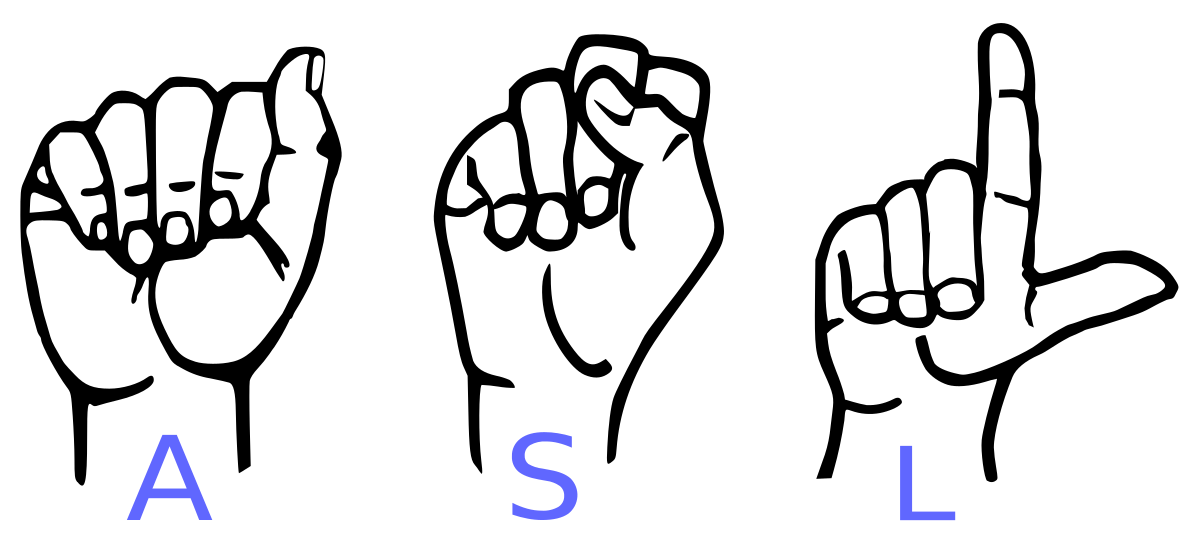
\includegraphics[height=%
0.29\textheight]{asl}\\
\subsection{Introduzione al Database}
Il \textbf{Linguaggio dei segni} è una delle modalità di comunicazione più usata per l'interazione con persone con difficoltà a parlare o a sentire. La maggioranza delle persone, però, non è in grado di comprenderne il significato. Questo linguaggio consiste nell'assegnazione ad ogni lettera dell'alfabero ad una specifica posizione della mano. Di conseguenza, per ogni diverso alfabeto, si vengono a delineare diversi linguaggi dei segni.\\
Quello che viene analizzato nello specifico in questo progetto è \textbf{American Sign Language}(ASL).

\subsection{Obiettivi}
Al fine di facilitare la comunicazione tra persone e abbattere il limite della conoscenza di questo specifico linguaggio, l'obiettivo principale del progetto è quello di realizzare un sistema automatico in grado di riconoscere  immagini relative al linguaggio dei segni e di tradurne il significato. \\
Lo scopo di questa ricerca è quindi quello di allenare un modello in grado di rilevare e riconoscere gesti e segni delle mani e di tradurli in lettere dell'alfabeto americano.
\newpage

\section{Preprocessing}
Ogni progetto di Computer Vision vede una prima fase fondamentale di \textbf{preprocessing} dei dati. \\
L'importanza di questa fase è dovuta alla necessità di istanziare una serie di funzioni atte alla preparazione dei dati in funzione dell'algoritmo che verrà utilizzato. Ogni algoritmo di detection e recognition necessita di uno specifico formato dei dati.\\
A tale scopo, dunque, sono state definite alcune funzioni utili tra cui:
\begin{itemize}
\item {\itshape parse\_txt\_annot}: una funzione per convertire file txt in liste
\item {\itshape create\_paths\_list}: una funzione per creare liste di file paths
\item {\itshape creating\_files}: una funzione per creare file nel formato dizionario
\end{itemize}
Ma prima di descriverne più dettagliatamente l'utilizzo, è importante capire il significato dei file txt.\\


Il processo di \textbf{Object Detection} restituisce una {\itshape bounding box}, l'etichetta della classe e spesso una probabilità (o score) per ogni oggetto di interesse presente nell'immagine di input. \\
Per ogni file (immagine) presente rispettivamente nella directory di train, validation e test si trova un corrispondente file testuale contenente le coordinate di una o più bounding box. Più precisamente, ad ogni immagine corrisponde un file con (necessariamente) lo stesso nome, ma diversa estensione (.txt). Il file testuale è suddiviso in righe e ad ogni righe corrispondono 4 valori separati da uno spazio.\\
\begin{itemize}
\item {\itshape bbox\_cat}: è il primo valore (intero) e indica la classe di appartenenza dell'oggetto individuato, definito da un'opportuna funzione di mapping;
\item {\itshape x}: indica l'ascissa relativa alle coordinate del centro di posizionamento della bounding box (può essere espressa in forma relativa o assoluta);
\item {\itshape y}: similmente a prima, è l'ordinata relativa al centro di posizionamento della bounding box (anch'essa, relativa o assoluta);
\item {\itshape width}: indica la lunghezza orizzontale relativa alla bounding box in oggetto;
\item {\itshape height}: indica, invece, l'altezza della bounding box
\end{itemize}
Questo file, quindi, contiene i dati per delineare i contorni di rilevamento degli oggetti nell'immagine e la loro categoria, appartenente ad un insieme definito.\\

\subsection{Parse\_txt\_annotation}
\begin{itemize}
\item La funzione legge una singola immagine e il relativo file txt associato e traduce le diverse coordinate in tre array. In particolare:
\begin{itemize}
\item dall'immagine: estrae le dimensioni, altezza e larghezza
\item dal file testuale: i 4 valori, per ogni riga, espresse in forma relativa
\end{itemize} 
Successivamente, calcola le coordinate assolute delle bounding box relativamente ai 4 angoli che delineano il rettangolo di rilevazione dell'oggetto nell'immagine (xmin,ymin,xmax,ymax). \\
La funzione ritorna, perciò, 3 liste:
\begin{itemize}
\item img\_path: indirizzo dell'immagine
\item classes: lista contenente le rispettive classi rilevate all'interno del file
\item boxes: i 4 valori assoluti di tutte le bounding boxes calcolate
\end{itemize} 
\end{itemize} 

\subsection{Creating\_files}
\begin{itemize}
\item La funzione consente la creazione di 3 RaggedTensor (image\_paths, classes, bbox).\\
Un {\itshape RaggedTensor} è un tensore con una o più dimensioni ragged (irregolari); dimensioni che possono assumere lunghezze diverse.\\
Più in generale, invece, un {\itshape Tensor} è un array multidimensionale con un tipo uniforme. Come caratteristica fondamentale hanno l'immutabilità: non puoi mai aggiornare il contenuto di un tensore, ma crearne solo uno nuovo.\\
Per ottenere questo, la funzione, utilizzando due liste, inizialmente create e contenenti tutti i percorsi relativi alle corrispondenti immagini e file testuali, per ciascuna immagine parsa il file txt associato da cui separa i valori di bounding box da quelli della classe.\\
La funzione restituisce dunque le informazioni associate ad ogni singola immagine e relative al: percorso, classe di appartenenza e bounding box.
\end{itemize}

\subsection{Creazione datasets}
A questo punto, è possibile procedere alla definizione dei datasets in formato compatibile con l'algoritmo di Detection che verrà successivamente utilizzato.
\begin{itemize}
\item
\subsubsection{Img\_preprocessing}
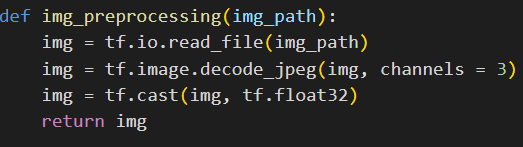
\includegraphics[height=%
0.1\textheight]{pp}\\
\begin{itemize}
\item {\itshape tf.io.read\_file(img\_path)}: utilizza TensorFlow per leggere il contenuto del file immagine specificato dal percorso img\_path e lo memorizza nella variabile img. Questo metodo restituisce i byte del file.

\item {\itshape tf.image.decode\_jpeg(img, channels=3)}: decodifica l'immagine JPEG rappresentata dai byte ottenuti dalla lettura del file. Il parametro channels=3 specifica che l'immagine verrà decodificata con 3 canali di colore (RGB). Il risultato è un tensore che rappresenta l'immagine con i suoi pixel e i relativi canali di colore.

\item {\itshape tf.cast(img, tf.float32)}: trasforma il tipo di dati dei pixel dell'immagine da interi (che di solito sono rappresentati da valori compresi tra 0 e 255) a float. Questa conversione è comune in molte operazioni di deep learning, poiché spesso si desidera eseguire calcoli con i pixel dell'immagine e i tipi di dati float sono più adatti per tali operazioni.

\end{itemize}
\end{itemize}

\begin{itemize}
\item
\subsubsection{Resizing}
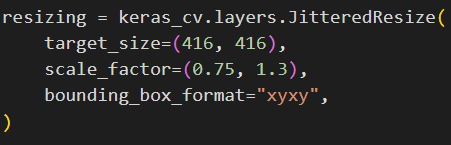
\includegraphics[height=%
0.1\textheight]{resize}\\
\begin{itemize}
\item La funzione {\itshape JitteredResize} esegue una ridimensionamento e jittering (sfocatura) casuale delle immagini in modo da aumentare la variabilità dei dati durante l'addestramento. Questo è utile per migliorare la capacità di generalizzazione del modello.
I parametri principali della classe sono:
\begin{itemize}
\item {\itshape target\_size}: specifica la dimensione target per l'immagine ridimensionata. In questo caso, le immagini vengono ridimensionate a una dimensione di 416x416 pixel.

\item {\itshape scale\_factor}: specifica il fattore di scala per il jittering casuale. Il jittering casuale viene applicato prima del ridimensionamento dell'immagine. In questo caso, il fattore di scala è impostato su (0.75,1.3), il che significa che le immagini vengono ridimensionate con un fattore di scala casuale compreso tra 0.75 e 1.3 lungo entrambi gli assi.

\item {\itshape bounding\_box\_format}: specifica il formato delle coordinate dei bounding box. In questo caso, è impostato su "xyxy", che indica che le coordinate dei bounding box sono rappresentate come coppie di coordinate (x\_min, y\_min, x\_max, y\_max).
\end{itemize}
In pratica, quando si utilizza questa funzione, le immagini di input vengono sottoposte a un jittering casuale seguito da un ridimensionamento al formato specificato. Questa tecnica può essere utile per migliorare la robustezza del modello durante l'addestramento, poiché esposta a una maggiore variabilità nei dati di input.

\end{itemize}
\end{itemize}

\begin{itemize}
\item
\subsubsection{Load dataset}
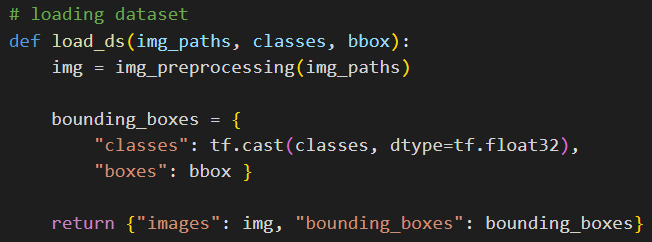
\includegraphics[height=%
0.18\textheight]{load}\\
\begin{itemize}
\item La funzione {\itshape Load\_ds} è progettata per caricare un dataset di immagini, con associate le relative classi e bounding boxes
\begin{itemize}
\item {\itshape img\_preprocessing(img\_paths)}: restituisce un tensore contenente l'immagine pre-elaborata.

\item {\itshape bounding\_boxes = \{"classes": tf.cast(classes, dtype=tf.float32), "boxes": bbox\}}: costruisce un dizionario (bounding\_boxes) che contiene le classi delle immagini e le relative bounding boxes. Le classi vengono convertite in float32 utilizzando tf.cast. 'classes' è un tensore delle classi corrispondenti all'immagine e 'bbox' è un tensore delle relative bounding boxes.

\end{itemize}
La funzione restituisce un dizionario contenente l'immagine pre-elaborata (img) e le informazioni sulle bounding boxes (bounding\_boxes). Questo dizionario sarà utilizzato per creare un batch di dati durante l'addestramento o la valutazione del modello.
\end{itemize}
\end{itemize}

\begin{itemize}
\item
\subsubsection{Dataset loaders}
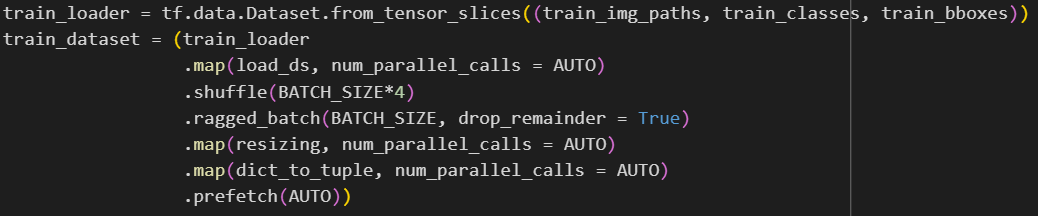
\includegraphics[height=%
0.15\textheight]{loader}\\
\begin{itemize}
\item {\itshape train\_loader}: è un oggetto (di tipo 'tf.data.Dataset') che viene creato utilizzando il metodo {\itshape from\_tensor\_slices}, prendendo in input una tupla di tensori ('train\_img\_paths', 'train\_classes', 'train\_bboxes'). Più precisamente, viene creato un dataset dove ogni elemento corrisponde ad una tupla contenente un elemento da ciascun tensore.
\item {\itshape train\_dataset}: è il dataset di addestramento completo, ottenuto a seguito di un pre-processing su {\itshape train\_loader}.\\
Ad esso, infatti, vengono applicate una serie di trasformazioni utilizzando specifici metodi della libreria TensorFlow: \textbf{map, shuffle, ragged\_batch,  e prefetch}. \\
In particolare:\\
\begin{itemize}
\item {\itshape map(load\_ds, num\_parallel\_calls = AUTO)}: applica la funzione 'load\_ds' ad ogni elemento del dataset in parallelo. \\
'num\_parallel\_calls = AUTO' indica a TensorFlow di utilizzare un numero di thread appropriato sulla base della capacità della CPU.

\item {\itshape shuffle(BATCH\_SIZE*4)}: effettua uno shuffle (mescolamento) sugli elementi del dataset utilizzando una dimensione di buffer di dimensione BATCH\_SIZE*4. Questa operazione è indispensabile al fine di evitare che l'algoritmo di addestramento impari correttamente sui dati.

\item {\itshape ragged\_batch(BATCH\_SIZE, drop\_remainder = True)}: raggruppa gli elementi del dataset in batch di dimensione BATCH\_SIZE, scartando eventuali elementi rimanenti se non sono sufficienti per formare un batch completo. L'opzione 'ragged\_batch' permette di gestire batch di dimensioni diverse.

\item {\itshape map(resizing, num\_parallel\_calls = AUTO)}: applica la funzione 'resizing' ad ogni elemento del dataset in parallelo.

\item {\itshape map(dict\_to\_tuple, num\_parallel\_calls = AUTO)}: applica la funzione 'dict\_to\_tuple' ad ogni elemento del dataset in parallelo.

\item {\itshape prefetch(AUTO)}: carica in memoria i dati in anticipo in modo asincrono per migliorare le prestazioni dell'addestramento. Lavorare su dati presenti sulla cache offre vantaggi sui tempi di esecuzione nettamente rilevanti.
\end{itemize}
\end{itemize}

\end{itemize}
\newpage

\section{Yolo Model}
\subsection{Algoritmo}
\textbf{YOLO}, acronimo di "You Only Look Once", è un popolare framework per l'{\itshape Object Detection} in immagini e video. È noto per la sua capacità di effettuare rilevamento di oggetti multipli in tempo reale con elevata accuratezza.\\
L'approccio di YOLO si differenzia da molti altri metodi di object detection in quanto considera il problema come un'unica regressione diretta. Piuttosto che dividere l'immagine in varie regioni di interesse e applicare il classificatore separatamente a ciascuna regione (come nel caso di metodi basati su regione, come R-CNN), YOLO suddivide l'immagine in una griglia e predice le bounding boxes e le probabilità di classe per ciascuna cella della griglia contemporaneamente. Viene definita anche {\itshape rete single-stage}.\\

Le caratteristiche principali di YOLO sono:
\begin{itemize}

\item
\textbf{Efficienza}: YOLO è noto per la sua efficienza e la sua capacità di effettuare il rilevamento di oggetti in tempo reale. Il suo approccio di "You Only Look Once" consente una {\itshape rapida} inferenza su singole immagini o flussi video.
\item
\textbf{Simultaneità}: YOLO effettua la predizione delle bounding boxes e delle probabilità di classe in un'unica passata attraverso la rete neurale. Questo lo rende {\itshape più veloce} rispetto ai metodi tradizionali che richiedono più passaggi per l'individuazione degli oggetti.

\item
\textbf{Buona generalizzazione}: YOLO generalizza bene su una vasta gamma di classi di oggetti e condizioni di illuminazione, grazie alla sua capacità di apprendere pattern spaziali e contestuali nell'immagine.

\item
\textbf{Open Source}: YOLO è un framework open source ed è disponibile in diverse versioni, ciascuna con miglioramenti e ottimizzazioni rispetto alla versione precedente. Nel progetto è stata utilizzata l'ultima versione, v8. Yolov8 è un algoritmo allo stato dell'arte.

\end{itemize}
YOLO è ampiamente utilizzato in applicazioni di sorveglianza, veicolari, di analisi video e in altri contesti in cui è necessario il rilevamento e la classificazione degli oggetti in tempo reale.

\subsection{Yolo v8}







\end{document}
